\documentclass[11pt,a4paper]{article}
\usepackage[T1]{fontenc}
\usepackage{lmodern,microtype}
\usepackage[hmargin=27mm,vmargin=22mm]{geometry}
\usepackage{amsmath,amssymb,amsthm,booktabs,tikz}
\usepackage[hidelinks]{hyperref}
\hypersetup{pdftitle={The sharp adjacency--Laplacian gap for connected graphs}}
\newtheorem{theorem}{Theorem}
\newcommand{\gap}{\mu_1-\lambda_2}
\newcommand{\proved}{\textsc{Proved.}}
\newcommand{\verified}{\textsc{Verified.}}
\setlength{\parindent}{0pt}
\setlength{\parskip}{4pt plus 1pt}
\allowdisplaybreaks[1]
\begin{document}

{\large\bfseries Verdict\quad SOLVED by disproof}\par
\vspace{7pt}
{\huge\bfseries The sharp adjacency--Laplacian\\[3pt]gap for connected graphs}\par
\vspace{6pt}
{\large A disproof of Cazenave's Conjecture 2}\par
{\small 10 November 2026}\par
\vspace{8pt}
\hrule
\vspace{8pt}

Cazenave asks whether the largest Laplacian eigenvalue $\mu_1$ and the second-largest adjacency eigenvalue $\lambda_2$ of every finite simple connected graph of order at least $2$ satisfy $\mu_1-\lambda_2\ge2$ \cite[\S7, Conjecture 2, corpus \#20829]{cazenave}.

\begin{theorem}[\proved]\label{thm:main}
For each integer $n\ge11$ there is a connected simple graph of order $n$ with
\[
\gap\le 2-\frac1{119}.
\]
For every connected simple graph of order at least $2$, $\gap>1$. The infimum of the gap over all such graphs is $1$.
\end{theorem}

\verified\ Exact arithmetic on all $11{,}989{,}763$ connected unlabeled graphs of orders $2$ through $10$ found that they satisfy the conjectured inequality. Together with the explicit witness, this determines the minimum counterexample order as $11$. The disproof and sharp constant have symbolic proofs independent of this enumeration.

\section{Notation and spectral tests}

Let $A$ be the adjacency matrix, $D$ the diagonal matrix of degrees, and $L=D-A$. We order eigenvalues decreasingly and count multiplicity. The largest eigenvalue of a real symmetric matrix $M$ is the maximum Rayleigh quotient $x^{\mathsf T}Mx/\|x\|^2$ over nonzero $x$. If the Rayleigh quotient of $A$ is at least $b$ on a two-dimensional space, then $\lambda_2\ge b$. The space contains a nonzero vector orthogonal to a top eigenvector, and its Rayleigh quotient is at most $\lambda_2$ by expansion in an orthonormal eigenbasis. For two nonzero trial vectors with disjoint supports and zero mixed adjacency form, the quotient of any linear combination is a weighted average of the individual quotients.

For any matrix $M$ and strictly positive weights $h_i$, every eigenvalue has absolute value at most
\begin{equation}\label{eq:rows}
\max_i\frac{\sum_j |M_{ij}|h_j}{h_i}.
\end{equation}
For a nonzero eigenvector $y$, choose an index maximizing $|y_i|/h_i$ and apply the triangle inequality to that row of $My=\lambda y$.

\section{A counterexample at every order from 11 upward}

\proved\ Take two copies of $K_4$ with vertices $u_i,v_i,w_{i1},w_{i2}$, for $i=1,2$. Delete $u_iv_i$ in each copy. Join $u_1$ and $u_2$ by a path with $b=n-8\ge3$ internal vertices $p_1,\ldots,p_b$. Each block is connected and the path meets both blocks.

\begin{center}
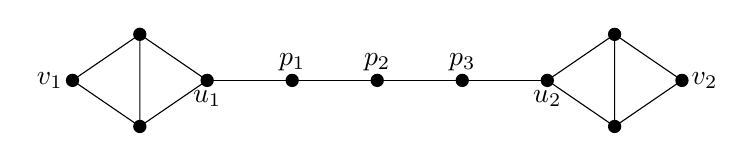
\begin{tikzpicture}[vertex/.style={circle,fill=black,inner sep=1.7pt},scale=.9]
\coordinate (u1) at (-2.4,0); \coordinate (v1) at (-4.3,0);
\coordinate (a1) at (-3.35,.65); \coordinate (b1) at (-3.35,-.65);
\coordinate (u2) at (2.4,0); \coordinate (v2) at (4.3,0);
\coordinate (a2) at (3.35,.65); \coordinate (b2) at (3.35,-.65);
\coordinate (p1) at (-1.2,0); \coordinate (p2) at (0,0); \coordinate (p3) at (1.2,0);
\foreach \i in {1,2} {\draw (u\i)--(a\i)--(v\i)--(b\i)--(u\i) (a\i)--(b\i);}
\draw (u1)--(p1)--(p2)--(p3)--(u2);
\foreach \v in {u1,v1,a1,b1,u2,v2,a2,b2,p1,p2,p3} {\node[vertex] at (\v) {};}
\node[below] at (u1) {$u_1$}; \node[left] at (v1) {$v_1$};
\node[below] at (u2) {$u_2$}; \node[right] at (v2) {$v_2$};
\node[above] at (p1) {$p_1$}; \node[above] at (p2) {$p_2$}; \node[above] at (p3) {$p_3$};
\end{tikzpicture}

\small The graph at order $11$ has $14$ edges. Subdivision of interior path edges gives the higher orders.
\end{center}

\textbf{Adjacency lower bound.} Assign weights $(3,3,4,4,1)$ to $(u_1,v_1,w_{11},w_{12},p_1)$ and zero elsewhere. Use the reflected assignment on the right with $p_b$ in place of $p_1$. Each squared norm is $51$. On either support the sum of the edge products is $4\cdot12+16+3=67$, so the adjacency form is $134$. Since $b\ge3$, the supports are disjoint and have no edge between them. Thus $\lambda_2\ge134/51$.

\textbf{Laplacian upper bound.} For each $i$, the vector supported on $w_{i1},w_{i2}$ with entries $1,-1$ is a Laplacian eigenvector of eigenvalue $4$. On the invariant orthogonal complement the two coordinates agree, with common value $w_i$. Use one coordinate per such pair, leaving all others separate. Taking absolute values in the resulting quotient $M$ gives the following rows. Here $p$ is a path vertex adjacent to a block, and $p'$ is the next path vertex.
\[
\begin{array}{c@{\quad}l@{\quad}r@{\quad}r}
\toprule
\text{Row}&\text{Action on nonnegative coordinates}&h_i&(|M|h)_i\\
\midrule
u&3u+2w+p&63&291\\
v&2v+2w&26&120\\
w&2w+u+v&34&157\\
p&2p+u+p'&34&157\\
\text{Interior path vertex}&2p_j+p_{j-1}+p_{j+1}&26&\le120\\
\bottomrule
\end{array}
\]
Both neighbors of an interior path vertex have weights at most $34$. The diagonal $2$ in the $w$ row accounts for cancellation of the edge joining the two equal coordinates. The bound in \eqref{eq:rows} is $97/21$, the maximum of $291/63$, $120/26$, and $157/34$, and it also covers the two eigenvalues $4$. Hence
\[
\gap\le\frac{97}{21}-\frac{134}{51}=\frac{237}{119}=2-\frac1{119}.
\]

\section{Counterexamples with a two-edge connecting path}

\proved\ Let $G_{k,s}$ consist of two $K_k$ blocks, with $s$ edges incident to a designated port $u_i$ deleted from block $i$, and a new vertex $z$ joined to both ports. Assume $1\le s\le k-2$, so the ports still have neighbors in their blocks. We prove that $G_{k,1}$ violates the conjecture for every $k\ge6$.

Write $r=k-2$ and denote by $v_i$ the other endpoint of the deleted edge. The vector on each block with weights $5$ on $u_i,v_i$ and $6$ on the $r$ ordinary vertices has adjacency Rayleigh quotient
\[
\frac{36r(r-1)+120r}{36r+50}
=r+\frac7{10}+\frac{88r-350}{10(36r+50)}>r+\frac7{10}.
\]
Extend each vector by zero, so the supports have no mutual edges. Thus $\lambda_2>k-13/10$.

The sum-zero coordinate subspace on the ordinary vertices of either block has Laplacian eigenvalue $k$. On its combined orthogonal complement use one coordinate $w_i$ for the ordinary vertices of each block. The absolute quotient rows act as
\[
(r+1)u_i+rw_i+z,\quad rv_i+rw_i,\quad 2w_i+u_i+v_i,\quad 2z+u_1+u_2.
\]
For $t=k+7/10$ use weights $h_{u_i}=25r+26$, $h_{v_i}=15r$, $h_{w_i}=40$, $h_z=54$. The four types of coordinates of $th-|M|h$ are
\[
\frac{25r-98}{10},\qquad \frac r2,\qquad 2,\qquad \frac{20r-71}{5}.
\]
All are positive for $r\ge4$. By \eqref{eq:rows}, $\mu_1<t$, which gives $\gap<2$.

\section{The optimal universal constant}

\proved\ For the lower bound, let $\Delta$ be the maximum degree. For any real vector $x$,
\[
x^{\mathsf T}Ax=2\sum_{uv\in E}x_u x_v\le\sum_v d(v)x_v^2\le\Delta\|x\|^2.
\]
If $\Delta$ is an adjacency eigenvalue, equality on every edge in $2x_ux_v\le x_u^2+x_v^2$ forces its eigenvectors to be constant by connectedness. Thus that eigenspace has dimension at most one and $\lambda_2<\Delta$. For the Laplacian use value $\Delta$ at a maximum-degree vertex, $-1$ on its neighbors and $0$ elsewhere. The norm squared is $\Delta(\Delta+1)$, and the incident edges alone contribute $\Delta(\Delta+1)^2$ to $x^{\mathsf T}Lx=\sum_{uv\in E}(x_u-x_v)^2$. Hence $\mu_1\ge\Delta+1$ and $\gap>1$.

For sharpness use $G_{k,s}$, with $k>2$. Indicators of the two blocks give $\lambda_2\ge k-1-2s/k$, since each block has $k(k-1)/2-s$ edges. Write $X$ for the vector of all block coordinates, $a_i$ for the port coordinate in block $i$, $b_{ij}$ for the $s$ coordinates of its deleted neighbors, and $z$ for the connector coordinate. A clique contributes $k\sum_v x_v^2-(\sum_v x_v)^2$ to the Laplacian form, by expansion. Put $q=1/s$. For each block, expansion using $sq=1$ gives
\begin{align*}
q\left(a_i^2+\sum_j b_{ij}^2\right)-a_i^2+\sum_j(a_i-b_{ij})^2
&=(1+q)\sum_j\left(b_{ij}-\frac{a_i}{1+q}\right)^2+\frac{q^2a_i^2}{1+q}\ge0.
\end{align*}
Drop the negative clique sums, subtract the deleted-edge energies, and add $(a_1-z)^2+(a_2-z)^2$. This gives
\[
x^{\mathsf T}Lx\le(k+q)\|X\|^2+2z^2-2z(a_1+a_2).
\]
Completing the square in $z$ gives
\[
-2z(a_1+a_2)\le(k-2)z^2+\frac{(a_1+a_2)^2}{k-2}\le(k-2)z^2+\frac{2\|X\|^2}{k-2}.
\]
Thus $\mu_1\le k+1/s+2/(k-2)$ and
\[
\gap\le 1+\frac{2s}{k}+\frac1s+\frac2{k-2}.
\]
Take $k=s^2$ and send the integer $s\ge2$ to infinity to obtain the infimum $1$. This completes the proof of Theorem~\ref{thm:main}.

\section{Computations and controls}

\verified\ A floating-point exploration tested all $576$ combinations of $3\le k\le50$, path length $1\le\ell\le6$, and $s\in\{0,1\}$ deleted edges per block. It classified violations at a computed gap below $2-10^{-10}$. With $s=1$ the first hits by path length were $(\ell,k)=(2,6),(3,5),(4,4),(5,4),(6,4)$. The $s=0$ and $\ell=1$ configurations gave zero hits. A deleted edge in the $K_2$ spectrum oracle forced the expected failure.

\verified\ A full-matrix rational check evaluated the trial quotients and the pivots of $tI-L$ for the order-$11$ graph and $G_{k,1}$ for $6\le k\le25$. It used $t=37/8$ at order $11$ and $t=k+7/10$ for the other graphs. Restoring the two deleted edges at order $11$ yielded a negative pivot $-115/8$. Adding an edge between the trial supports made their mixed adjacency form $1$, which the checker rejected. See \texttt{compute.py}.

\verified\ The \texttt{geng} generator from nauty enumerated connected unlabeled graphs at each order $2\le n\le10$ \cite{nauty}. The verifier first tried interlacing. Deleting a vertex whose closed neighborhood contains every maximum-degree vertex gives maximum degree at most $\Delta-1$ in the principal subgraph, hence $\lambda_2\le\Delta-1$. Otherwise it tried a rational threshold $p/q$ with at most one negative eigenvalue of $pI-qA$ and either $p/q\le\Delta-1$ or a negative eigenvalue of $(p+2q)I-qL$. These conditions imply the conjectured bound by the star estimate or the inertia test. Fraction-free elimination counted negative pivots, marking a zero pivot inconclusive at that threshold. The three methods certified $11{,}807{,}037$, $181{,}616$, and $1{,}110$ graphs, respectively, with $0$ unresolved. A planted pivot-sign error failed the exact $K_2$ inertia test. The verifier also rejected the known order-$11$ counterexample. See \texttt{run\_small\_orders.sh} and \texttt{small\_orders.log}.

\section{What is not established}

The minimum-order result depends on exact enumeration through order $10$. The sharp constant is an infimum, and the strict lower bound excludes attainment. The construction gives sufficient families of counterexamples. Classification of all violations or of sequences approaching the infimum remains open in this analysis.

\appendix
\section{Dead ideas and route ledger}

\begin{itemize}
\item \textbf{Maximum degree alone.} The star Rayleigh vector and the adjacency row bound give a gap of $1$. The sharp family proves that this method's constant is already optimal for the unrestricted class.
\item \textbf{Complete blocks and direct one-edge joins.} The grid gave no violation with complete blocks or with a direct join and one deletion per block. A degree-two connector changed the Laplacian contribution while keeping the trial adjacency supports nonadjacent.
\item \textbf{Absolute row bound on the full Laplacian.} The unscaled bound $2\Delta$ grows too quickly on dense blocks. Passing to the quotient first retains the cancellation inside each clique, after which positive weights control the remaining rows.
\item \textbf{Floating-point and random searches.} Numerical signs are insufficient for a strict spectral certificate or a minimum-order claim. The proofs use two-dimensional Rayleigh spaces, exact quotient bounds, and a sum of squares. Exact inertia handles the finite exclusion. Number-theoretic sieves supply no input for these graph certificates.
\end{itemize}

\begin{thebibliography}{2}
\bibitem{cazenave} Tristan Cazenave, \emph{Lemmas and Conjectures in Spectral Graph Theory}, arXiv:2611.03879v1, 2 November 2026. \url{https://arxiv.org/abs/2611.03879v1}.
\bibitem{nauty} Brendan D. McKay and Adolfo Piperno, \emph{Practical graph isomorphism, II}, J. Symbolic Comput. 60 (2014), 94--112. \url{https://arxiv.org/abs/1301.1493}. Generator documentation at \url{https://users.cecs.anu.edu.au/~bdm/nauty/}.
\end{thebibliography}

\end{document}
